\chapter{Plane Electromagnetic Waves and Polarization}\label{ch:b2:plane-waves-polarization}

Tilt your head while wearing polarizing sunglasses and the glare on the
wet road comes and goes; turn the glasses in front of a phone screen
and the screen goes black. The light that reaches your eye is not only
a wave with a frequency and an intensity: it has a \emph{direction of
vibration}, and every polarizer, screen, 3D-cinema lens and optical
fibre connector plays with it. This chapter solves \omterm{thm:b2:maxwell-equations:maxwell}{Maxwell's equations}
in empty space --- the plane wave, with its transverse electric and
magnetic fields locked at right angles --- surveys the spectrum those
waves span, and studies the polarization: how to describe it, how to
select it with a polarizer (\omterm{prop:b2:plane-waves-polarization:malus}{Malus's law}), and how to transform it with
a birefringent plate.

\section{Plane waves in vacuum}

\begin{theorem}[Wave equation; plane progressive harmonic waves]\label{thm:b2:plane-waves-polarization:wave}
\index{electromagnetic wave}\index{plane wave (electromagnetic)}\index{transversality}
In vacuum, free of charges and currents, \omterm{thm:b2:maxwell-equations:maxwell}{Maxwell's equations} give
\[
\Delta\vect E = \frac1{c^2}\frac{\partial^2\vect E}{\partial t^2} , \qquad
\Delta\vect B = \frac1{c^2}\frac{\partial^2\vect B}{\partial t^2} , \qquad
c = \frac1{\sqrt{\varepsilon_0\mu_0}} = \qty{2.998e8}{m/s} .
\]
The \emph{plane progressive harmonic wave} (PPH wave) $\underline{\vect E} =
\underline{\vect E}_0\,\eu^{\iu(\omega t - \vect k\cdot\vect r)}$ is a solution provided
$\omega = ck$ (no dispersion), and \omterm{thm:b2:maxwell-equations:maxwell}{Maxwell's equations} then require
\[
\vect k\cdot\vect E = 0 , \qquad
\vect B = \frac{\vect k\wedge\vect E}\omega = \frac{\vect u\wedge\vect E}c ,
\]
$\vect u = \vect k/k$ being the direction of propagation: the wave is
\emph{transverse}, $(\vect E, \vect B, \vect u)$ is a right-handed orthogonal
triad, $\vect E$ and $\vect B$ are in phase and $B = E/c$. Its intensity is
$I = \varepsilon_0cE_0^2/2$ and it carries the \omterm{thm:b2:flow-balances:momentum}{momentum flux} $I/c$
(\cref{ch:b2:poynting-vector}).
\end{theorem}

\begin{proof}
The \omterm{thm:b2:waves-on-strings:equation}{wave equation} was derived in \cref{exo:b2:maxwell-equations:11}.
For $\eu^{\iu(\omega t - \vect k\cdot\vect r)}$, $\partial_t \to \iu\omega$ and $\vect\nabla \to
-\iu\vect k$: $\Delta \to -k^2$, so $k^2 = \omega^2/c^2$; Maxwell--Gauss gives $-\iu
\vect k\cdot\underline{\vect E} = 0$, Maxwell--flux $\vect k\cdot\underline{\vect B} = 0$,
Maxwell--Faraday $-\iu\vect k\wedge\underline{\vect E} = -\iu\omega\underline{\vect B}$, whence
$\underline{\vect B} = \vect k\wedge\underline{\vect E}/\omega$, of modulus $kE/\omega = E/c$ and
perpendicular to both; Maxwell--Ampère is then satisfied identically.
\end{proof}

\begin{omfigure}
\begin{tikzpicture}[font=\small, x=1cm, y=1cm, >=Stealth]
  \draw[->, thick] (-0.3,0) -- (7.4,0) node[right, font=\footnotesize] {$\vect u$};
  \draw[omDef, thick, domain=0:6.8, samples=80] plot (\x,{1.1*cos(deg(1.2*\x))});
  \draw[omProp, thick, domain=0:6.8, samples=80] plot (\x,{-0.4*cos(deg(1.2*\x))});
  \foreach \x in {0,0.65,...,6.6} {
    \pgfmathsetmacro{\e}{1.1*cos(deg(1.2*\x))}
    \draw[omDef, ->] (\x,0) -- (\x,\e);
    \draw[omProp, ->] (\x,0) -- ({\x+0.55*\e*0.36},{-0.4*\e*0.9});
  }
  \node[omDef, font=\footnotesize] at (0.4,1.45) {$\vect E$}; \node[omProp, font=\footnotesize] at (0.9,-0.75) {$\vect B = \vect u\wedge\vect E/c$};
  \draw[<->] (0,-1.3) -- (5.24,-1.3) node[midway, below, font=\footnotesize] {$\lambda = 2\pi/k = c/f$};
\end{tikzpicture}

{\small A plane progressive harmonic wave at one instant: $\vect E$ and
$\vect B$ perpendicular to each other and to the direction of travel, in
phase, $B = E/c$; the whole pattern slides along $\vect u$ at $c$.}
\end{omfigure}

\begin{remark}[The spectrum]\label{rem:b2:plane-waves-polarization:spectrum}
\index{electromagnetic spectrum}
One equation, one speed, and twenty orders of magnitude of frequency.
Radio: \qty{30}{kHz}--\qty{300}{MHz} ($\lambda$ from \qty{10}{km} to \qty{1}{m}),
antennas and circuits (\cref{ch:b2:dipole-radiation}). Microwaves:
\qty{300}{MHz}--\qty{300}{GHz}, radar, ovens, mobile phones, the cosmic
background. Infrared: to \qty{400}{THz} (\qty{750}{nm}), the thermal
radiation of everything around us (\cref{ch:b2:thermal-radiation}).
Visible: \qty{400}{THz}--\qty{750}{THz}, \qty{750}{nm} (red) to \qty{400}{nm}
(violet) --- one octave, photons of $1.6$ to \qty{3.1}{eV}. Ultraviolet to
\qty{10}{nm}; X-rays to \qty{10}{pm} (\qty{100}{keV}), from inner atomic shells
and braking electrons; gamma rays beyond, from nuclei. Only the sources
and the detectors differ: the wave is the same.
\end{remark}

\begin{omfigure}
\begin{tikzpicture}[font=\small, x=1cm, y=1cm, >=Stealth]
  \draw[->, thick] (0,0) -- (13.2,0) node[right, font=\footnotesize] {$f$};
  \foreach \x/\l in {0/$10^4$, 2/$10^6$, 4/$10^8$, 6/$10^{10}$, 8/$10^{12}$, 10/$10^{14}$, 12/$10^{16}$} {
    \draw (\x,-0.1) -- (\x,0.1); \node[font=\scriptsize, below] at (\x,-0.12) {\l};
  }
  \node[font=\scriptsize, below] at (13.0,-0.12) {Hz};
  \fill[omDef!30] (0,0.3) rectangle (4.5,1.0); \node[font=\footnotesize] at (2.25,0.65) {radio};
  \fill[omDef!50] (4.5,0.3) rectangle (7.5,1.0); \node[font=\footnotesize] at (6.0,0.65) {microwaves};
  \fill[omThm!30] (7.5,0.3) rectangle (10.6,1.0); \node[font=\footnotesize] at (9.05,0.65) {infrared};
  \fill[omProp!60] (10.6,0.3) rectangle (10.9,1.0);
  \fill[omThm!60] (10.9,0.3) rectangle (12.5,1.0); \node[font=\footnotesize] at (11.7,0.65) {UV};
  \fill[omExo!50] (12.5,0.3) rectangle (13.2,1.0); \node[font=\footnotesize] at (12.85,0.65) {X, $\gamma$};
  \node[font=\scriptsize, omProp] at (10.75,1.3) {visible};
  \node[font=\scriptsize] at (1.0,1.45) {$\lambda = \qty{30}{km}$}; \node[font=\scriptsize] at (6.0,1.45) {\qty{3}{cm}}; \node[font=\scriptsize] at (10.75,1.75) {\qty{600}{nm}}; \node[font=\scriptsize] at (12.5,1.45) {\qty{10}{nm}};
\end{tikzpicture}

{\small The \omterm{rem:b2:plane-waves-polarization:spectrum}{electromagnetic spectrum} on a logarithmic frequency scale;
the visible band is a sliver --- one octave out of twenty decades.}
\end{omfigure}

\section{Polarization}

\begin{definition}[Polarization states]\label{def:b2:plane-waves-polarization:states}
\index{polarization (of light)}\index{linear polarization}\index{circular polarization}\index{elliptical polarization}\index{natural light}
For a PPH wave along $z$ the field in a plane $z = $ const is
\[
\vect E = E_{0x}\cos(\omega t - kz)\,\vect e_x + E_{0y}\cos(\omega t - kz - \varphi)\,\vect e_y ,
\]
and the tip of $\vect E$ describes, in general, an ellipse: \emph{elliptical
polarization}. Two special cases: $\varphi = 0$ or $\pi$, \emph{linear}
polarization along a fixed direction at angle $\arctan(\pm E_{0y}/E_{0x})$
from $x$; $E_{0x} = E_{0y}$ and $\varphi = \pm\pi/2$, \emph{circular}
polarization, $\vect E$ of constant modulus turning at $\omega$ (right or
left according to its sense of rotation, seen facing the oncoming
wave). \emph{Natural} (unpolarized) light, from a lamp or the Sun, is
a succession of short wave trains with random, rapidly changing
polarizations: no direction is preferred on average. Any polarization
decomposes into two linear (or two circular) components.
\end{definition}

\begin{proof}
With $X = E_x/E_{0x}$, $Y = E_y/E_{0y}$: $X = \cos\theta$, $Y = \cos(\theta - \varphi)$, so
$X^2 + Y^2 - 2XY\cos\varphi = \sin^2\varphi$, an ellipse, degenerate into the
lines $Y = \pm X$ for $\varphi = 0, \pi$ and into a circle for $E_{0x} = E_{0y}$,
$\varphi = \pm\pi/2$.
\end{proof}

\begin{proposition}[Polarizers and Malus's law]\label{prop:b2:plane-waves-polarization:malus}
\index{polarizer}\index{Malus's law}\index{analyser}
A \emph{polarizer} transmits the component of $\vect E$ along its
transmission axis $\vect p$ and absorbs the other (a sheet of aligned
long molecules, which conduct along their length --- the transmitted
polarization is perpendicular to the molecules). Linearly polarized
light of intensity $I_0$ whose direction makes the angle $\theta$ with
$\vect p$ emerges linearly polarized along $\vect p$ with
\[
I = I_0\cos^2\theta \qquad\text{(Malus)} ;
\]
\omterm{def:b2:plane-waves-polarization:states}{natural light} emerges with $I_0/2$, polarized along $\vect p$. Two
crossed polarizers transmit nothing; a third one inserted at
\qty{45}{\degree} between them transmits $I_0/8$.
\end{proposition}

\begin{proof}
The transmitted amplitude is $E_0\cos\theta$ and $I \propto E_0^2$. \omterm{def:b2:plane-waves-polarization:states}{Natural
light}: average of $\cos^2\theta$ over all $\theta$, $\tfrac12$. Three polarizers:
$\tfrac12\cdot\cos^2 45^\circ\cdot\cos^2 45^\circ = \tfrac18$ --- the middle
polarizer does not merely attenuate, it \emph{turns} the polarization.
\end{proof}

\begin{omfigure}
\begin{tikzpicture}[font=\small, x=1cm, y=1cm, >=Stealth]
  \begin{scope}
    \draw[->, thick] (-0.4,0) -- (7.2,0) node[right, font=\footnotesize] {$z$};
    \foreach \x/\a/\l in {1.0/90/$\vect p_1$, 3.5/45/$\vect p_2$, 6.0/0/$\vect p_3$} {
      \draw[thick, fill=omExo!15] (\x,0) ellipse (0.35 and 1.1);
      \draw[omThm, very thick, <->] ({\x-0.3*cos(\a)},{-0.9*sin(\a)}) -- ({\x+0.3*cos(\a)},{0.9*sin(\a)});
      \node[omThm, font=\footnotesize] at (\x,1.4) {\l};
    }
    \node[font=\footnotesize] at (2.25,-1.5) {$I_0/2$}; \node[font=\footnotesize] at (4.75,-1.5) {$I_0/4$}; \node[font=\footnotesize] at (6.9,-1.5) {$I_0/8$};
    \node[font=\footnotesize] at (0.2,-1.5) {$I_0$, natural};
  \end{scope}
  \begin{scope}[xshift=10.2cm]
    \begin{axis}[omaxis, axis x line=bottom, axis y line=left, width=4.6cm, height=3.8cm, at={(0,-1.6cm)},
        xlabel={$\theta$}, ylabel={$I/I_0$}, xmin=0, xmax=180, ymin=0, ymax=1.1, xtick={0,90,180}, xticklabels={$0$, $90^\circ$, $180^\circ$}, ytick={0.5,1}, samples=100,
        xlabel style={at={(axis description cs:1.0,0.0)}, anchor=west},
        ylabel style={at={(axis description cs:-0.12,0.5)}, rotate=90, anchor=south}]
      \addplot[omDef, thick, domain=0:180] {cos(x)^2};
    \end{axis}
  \end{scope}
\end{tikzpicture}

{\small Left: \omterm{def:b2:plane-waves-polarization:states}{natural light} through three polarizers at $0^\circ$, $45^\circ$
and $90^\circ$ --- the middle one lets an eighth through a pair that
alone would block everything. Right: \omterm{prop:b2:plane-waves-polarization:malus}{Malus's law}.}
\end{omfigure}

\begin{example}[Sunglasses, screens, photographs]\label{ex:b2:plane-waves-polarization:uses}
Light reflected at a glancing angle from water or asphalt is largely
polarized horizontally (Brewster's angle, \cref{ch:b2:wave-interfaces}):
sunglasses with a vertical transmission axis cut the glare and keep the
rest. A liquid-crystal screen emits polarized light: through a
polarizer at \qty{90}{\degree} it goes black. A photographer's polarizing
filter darkens the sky (scattered light is partly polarized,
\cref{ch:b2:dipole-radiation}) and removes reflections from glass.
\end{example}

\section{Birefringence and wave plates}

\begin{proposition}[Wave plates]\label{prop:b2:plane-waves-polarization:plates}
\index{birefringence}\index{wave plate}\index{half-wave plate}\index{quarter-wave plate}\index{fast axis}\index{slow axis}
In a \emph{birefringent} crystal (calcite, quartz, mica; also a
stretched plastic sheet) a wave propagating along a given direction
splits into two \omterm{def:b2:plane-waves-polarization:states}{linear polarizations}, along the \emph{fast} and
\emph{slow} axes of the plate, travelling with different indices $n_f <
n_s$ (admitted --- the crystal responds differently along its axes). A
plate of thickness $e$ delays the slow component by the phase
\[
\delta = \frac{2\pi}\lambda(n_s - n_f)\,e .
\]
A \emph{\omterm{prop:b2:plane-waves-polarization:plates}{half-wave plate}} ($\delta = \pi$) turns a \omterm{def:b2:plane-waves-polarization:states}{linear polarization} at
angle $\alpha$ from the \omterm{prop:b2:plane-waves-polarization:plates}{fast axis} into a \omterm{def:b2:plane-waves-polarization:states}{linear polarization} at $-\alpha$: it
rotates it by $2\alpha$. A \emph{\omterm{prop:b2:plane-waves-polarization:plates}{quarter-wave plate}} ($\delta = \pi/2$) turns a
\omterm{def:b2:plane-waves-polarization:states}{linear polarization} at \qty{45}{\degree} from its axes into circular light,
and circular light back into linear; at other angles, into elliptical
light with axes along the plate's.
\end{proposition}

\begin{proof}
Write the incident field $E_0(\cos\alpha\,\vect e_f + \sin\alpha\,\vect e_s)\cos\omega t$;
after the plate, $E_0[\cos\alpha\cos\omega t\,\vect e_f + \sin\alpha\cos(\omega t - \delta)
\vect e_s]$. For $\delta = \pi$ the $\vect e_s$ component changes sign: direction
$(\cos\alpha, -\sin\alpha)$. For $\delta = \pi/2$ and $\alpha = 45^\circ$: $(E_0/\sqrt2)(\cos
\omega t, \sin\omega t)$, a circle.
\end{proof}

\begin{omfigure}
\begin{tikzpicture}[font=\small, x=1cm, y=1cm, >=Stealth]
  \begin{scope}
    \draw[->] (-1.5,0) -- (1.5,0) node[right, font=\footnotesize] {$x$}; \draw[->] (0,-1.5) -- (0,1.5) node[above, font=\footnotesize] {$y$};
    \draw[omDef, very thick, <->] (-1.1,-0.8) -- (1.1,0.8); \node[omDef, font=\footnotesize] at (1.25,1.05) {linear};
    \node[font=\footnotesize] at (0,-1.9) {$\varphi = 0$};
  \end{scope}
  \begin{scope}[xshift=4.2cm]
    \draw[->] (-1.5,0) -- (1.5,0); \draw[->] (0,-1.5) -- (0,1.5);
    \draw[omDef, very thick, postaction={decorate, decoration={markings, mark=at position 0.3 with {\arrow{>}}}}] (0,0) circle (1.0);
    \node[omDef, font=\footnotesize] at (1.25,1.15) {circular};
    \node[font=\footnotesize] at (0,-1.9) {$E_{0x} = E_{0y}$, $\varphi = \pm\pi/2$};
  \end{scope}
  \begin{scope}[xshift=8.4cm]
    \draw[->] (-1.5,0) -- (1.5,0); \draw[->] (0,-1.5) -- (0,1.5);
    \draw[omDef, very thick, rotate=30, postaction={decorate, decoration={markings, mark=at position 0.3 with {\arrow{>}}}}] (0,0) ellipse (1.2 and 0.55);
    \node[omDef, font=\footnotesize] at (1.3,1.15) {elliptical};
    \node[font=\footnotesize] at (0,-1.9) {general $\varphi$};
  \end{scope}
  \begin{scope}[xshift=12.4cm]
    \draw[thick, fill=omExo!15] (0,0) ellipse (0.35 and 1.3);
    \draw[omThm, thick, ->] (0,0) -- (0,1.0) node[right, font=\footnotesize, yshift=-3pt] {slow};
    \draw[omThm, thick, ->] (0,0) -- (0.5,0) node[right, font=\footnotesize] {fast};
    \node[font=\footnotesize] at (0,-1.9) {$\delta = 2\pi(n_s - n_f)e/\lambda$};
  \end{scope}
\end{tikzpicture}

{\small The polarization states of a plane wave, seen facing the
oncoming light, and a birefringent plate with its fast and slow axes.}
\end{omfigure}

\begin{example}[Where plates are used]\label{ex:b2:plane-waves-polarization:plateuses}
A \omterm{prop:b2:plane-waves-polarization:plates}{quarter-wave plate} between a polarizer and a mirror makes an
\emph{optical isolator}: the light goes out circular, comes back
circular of the opposite handedness, is turned by the plate into linear
light at \qty{90}{\degree} from the polarizer and is absorbed --- no
reflection returns to the laser. The two eyes' images of a 3D film are
projected in opposite \omterm{def:b2:plane-waves-polarization:states}{circular polarizations} and sorted by the
quarter-wave--polarizer sandwiches of the glasses, which still work
when you tilt your head (linear polarizers would not). A transparent
ruler between crossed polarizers shows coloured fringes: stress makes
plastic birefringent, and engineers read the stresses of a model from
the pattern.
\end{example}

\begin{method}[Following a polarization through optics]\label{met:b2:plane-waves-polarization:method}
(1) Choose axes; write the incident field as two components with
their phase difference. (2) A polarizer: keep the projection on its
axis (amplitude $\times\cos$, intensity $\times\cos^2$; \omterm{def:b2:plane-waves-polarization:states}{natural light}
$\times\tfrac12$). (3) A plate: project on its fast and slow axes, delay
the slow one by $\delta$, recombine. (4) Read the result: phase $0$ or $\pi$
means linear, $\pm\pi/2$ with equal amplitudes means circular. (5) To
test an unknown beam: rotate a polarizer (intensity varies: linear or
elliptical part), then add a \omterm{prop:b2:plane-waves-polarization:plates}{quarter-wave plate} (circular becomes
linear and can be extinguished).
\end{method}

\section{Exercises}

\begin{exercise}[$\star$]\label{exo:b2:plane-waves-polarization:1}
An FM station at \qty{100}{MHz} gives, at a receiver, an intensity of
\qty{1.0}{\micro W/m^2}. Wavelength, wavenumber, period; amplitudes $E_0$ and
$B_0$; energy density; emf induced in a \qty{1}{m} antenna aligned with
$\vect E$; photon flux (per square metre and second).
\end{exercise}

\begin{exercise}[$\star$]\label{exo:b2:plane-waves-polarization:2}
Frequency and photon energy (in eV) for $\lambda = \qty{1}{km}$, \qty{10}{cm},
\qty{10}{\micro m}, \qty{550}{nm}, \qty{10}{nm}, \qty{0.1}{nm}, \qty{1}{pm}; name the
band of each; the wavelength of a \qty{1}{MeV} gamma ray and of the
\qty{2.7}{K} cosmic background (peak near \qty{160}{GHz}).
\end{exercise}

\begin{exercise}[$\star$]\label{exo:b2:plane-waves-polarization:3}
Linearly polarized light of intensity $I_0$ falls on a polarizer at
\qty{30}{\degree}, then a second at \qty{60}{\degree} from the first, then a
third at \qty{90}{\degree} from the first: intensity after each. Same with
\omterm{def:b2:plane-waves-polarization:states}{natural light}. Remove the middle one: what changes?
\end{exercise}

\begin{exercise}[$\star$]\label{exo:b2:plane-waves-polarization:4}
Check that $\vect E = E_0\cos(\omega t - kz)\,\vect e_x$, $\vect B = (E_0/c)\cos(\omega t
- kz)\,\vect e_y$ satisfies the four Maxwell equations in vacuum when $\omega =
kc$. Which equation fixes the direction of $\vect B$, which its
magnitude? What happens if one tries $\vect E$ along $\vect e_z$?
\end{exercise}

\begin{exercise}[$\star\star$]\label{exo:b2:plane-waves-polarization:5}
\emph{Circular light.} (a) Write the field of a circularly polarized
wave along $z$ and show that $|\vect E|$ is constant while its direction
turns at $\omega$. (b) Show that the sum of a right- and a left-circular
wave of equal amplitudes is linearly polarized, along a direction set by
their relative phase. (c) Through a polarizer, what does circular light
give, and does the intensity depend on the polarizer's angle? (d) How
then can one tell circular light from \omterm{def:b2:plane-waves-polarization:states}{natural light}?
\end{exercise}

\begin{exercise}[$\star\star$]\label{exo:b2:plane-waves-polarization:6}
Quartz has $n_s - n_f = 0.0091$ at \qty{589}{nm}. (a) Thickness of a
\omterm{prop:b2:plane-waves-polarization:plates}{quarter-wave plate} of lowest order; of a \omterm{prop:b2:plane-waves-polarization:plates}{half-wave plate}. (b) A
\omterm{prop:b2:plane-waves-polarization:plates}{quarter-wave plate} for \qty{589}{nm} used at \qty{450}{nm}: phase delay
(neglect the variation of the indices); what comes out for linear light
at \qty{45}{\degree}? (c) Why are "multiple-order" plates (thickness $e +
m\lambda/(n_s - n_f)$) more sensitive to wavelength and temperature? (d) Why
must a plate's thickness be controlled to better than a micrometre?
\end{exercise}

\begin{exercise}[$\star\star$]\label{exo:b2:plane-waves-polarization:7}
\omterm{prop:b2:plane-waves-polarization:plates}{Half-wave plate}. (a) Show that linear light at angle $\alpha$ from the
\omterm{prop:b2:plane-waves-polarization:plates}{fast axis} comes out linear at $-\alpha$. (b) Hence a plate rotated by $\beta$
rotates the polarization by $2\beta$: what rotation of the plate turns a
vertical polarization horizontal? (c) What does a \omterm{prop:b2:plane-waves-polarization:plates}{half-wave plate} do to
circular light? (d) Between crossed polarizers, a \omterm{prop:b2:plane-waves-polarization:plates}{half-wave plate} is
rotated slowly: sketch the transmitted intensity against its angle.
\end{exercise}

\begin{exercise}[$\star\star$]\label{exo:b2:plane-waves-polarization:8}
$N$ polarizers are placed one after the other, each rotated by
$\pi/2N$ from the previous one, the last being at \qty{90}{\degree} from the
first. Transmission of linearly polarized light aligned with the first
for $N = 1, 2, 5, 10, 100$; limit $N \to \infty$ (use $\cos^{2N}(\pi/2N) \approx
1 - \pi^2/4N$). Comment: a polarization can be turned by \qty{90}{\degree}
with no loss --- by what?
\end{exercise}

\begin{exercise}[$\star\star$]\label{exo:b2:plane-waves-polarization:9}
\emph{Partial polarization.} A rotating polarizer in front of a beam
gives a maximum intensity $I_{\max}$ and a minimum $I_{\min}$. (a) Model the
beam as \omterm{def:b2:plane-waves-polarization:states}{natural light} $I_n$ plus linearly polarized light $I_p$: express
$I_{\max}$ and $I_{\min}$; the degree of polarization $p = I_p/(I_n + I_p) =
(I_{\max} - I_{\min})/(I_{\max} + I_{\min})$. (b) Blue sky at \qty{90}{\degree} from
the Sun: $I_{\max}/I_{\min} = 5$: $p$. (c) Light reflected from a lake near
Brewster's angle, $p = 0.9$: how much can polarizing sunglasses remove?
(d) Can a polarizer alone distinguish partially linearly polarized
light from partially circular light? What is needed?
\end{exercise}

\begin{exercise}[$\star\star\star$]\label{exo:b2:plane-waves-polarization:10}
\emph{Two crossed beams.} Two PPH waves of equal amplitude and
frequency, both polarized along $\vect e_y$, propagate in the $xz$ plane
at angles $\pm\theta$ from $z$. (a) Write the total field and show it is a
wave travelling along $z$ whose amplitude is modulated along $x$ as
$\cos(kx\sin\theta)$. (b) Spacing of the dark planes (interference
fringes); numbers for $\lambda = \qty{633}{nm}$, $\theta = \qty{5}{\degree}$, and for
$\theta = \qty{90}{\degree}$ (counter-propagating). (c) \omterm{def:b2:dispersion-wave-packets:relation}{Phase velocity} of the
pattern along $z$; compare with $c$; is anything travelling faster than
light? (d) Compute the time-averaged \omterm{thm:b2:poynting-vector:poynting}{Poynting vector} and show that its
$x$ component vanishes: the energy flows along $z$ in the bright
planes.
\end{exercise}

\begin{exercise}[$\star\star\star$]\label{exo:b2:plane-waves-polarization:11}
\emph{The liquid-crystal pixel.} A twisted-nematic cell between
crossed polarizers rotates the polarization of light by \qty{90}{\degree}
when no voltage is applied (the molecules' alignment twists through
the cell and the polarization follows it --- admitted), and not at all
when a few volts untwist them. (a) Transmission in both states: which
one is bright? (b) Real cells rotate by $90^\circ \pm 5^\circ$ at the design
wavelength: contrast ratio $I_{\text{bright}}/I_{\text{dark}}$ if the dark
state leaks through a residual \qty{5}{\degree} error. (c) Why does a cell
designed for \qty{550}{nm} leak some blue and red in the dark state
(think of the rotation as a stack of many thin half-wave-like
retarders)? (d) A colour pixel uses three such cells with filters; why
does the screen go black through a polarizer at some angle, and what
does that angle tell you?
\end{exercise}

\begin{exercise}[$\star\star\star$]\label{exo:b2:plane-waves-polarization:12}
\emph{Optical activity.} In a sugar solution the two \omterm{def:b2:plane-waves-polarization:states}{circular
polarizations} travel with slightly different indices $n_L$ and $n_R$.
(a) Decompose a \omterm{def:b2:plane-waves-polarization:states}{linear polarization} into circular components and show
that after a length $\ell$ the polarization is still linear but rotated
by $\theta = \pi(n_L - n_R)\ell/\lambda$. (b) A \qty{1}{dm} tube of a \qty{0.10}{g/mL}
sucrose solution rotates sodium light by \qty{6.65}{\degree}: $n_L - n_R$. (c)
A saccharimeter measures $\theta$ to \qty{0.01}{\degree}: precision on the
concentration. (d) The same effect is produced in glass by a magnetic
field along the beam (Faraday effect, $\theta = VB\ell$ with $V \approx
\qty{4}{rad.T^{-1}.m^{-1}}$): why does a Faraday rotator, unlike a sugar
tube, not cancel its rotation when the light is sent back, and how
does that make an isolator?
\end{exercise}

\begin{omfigure}
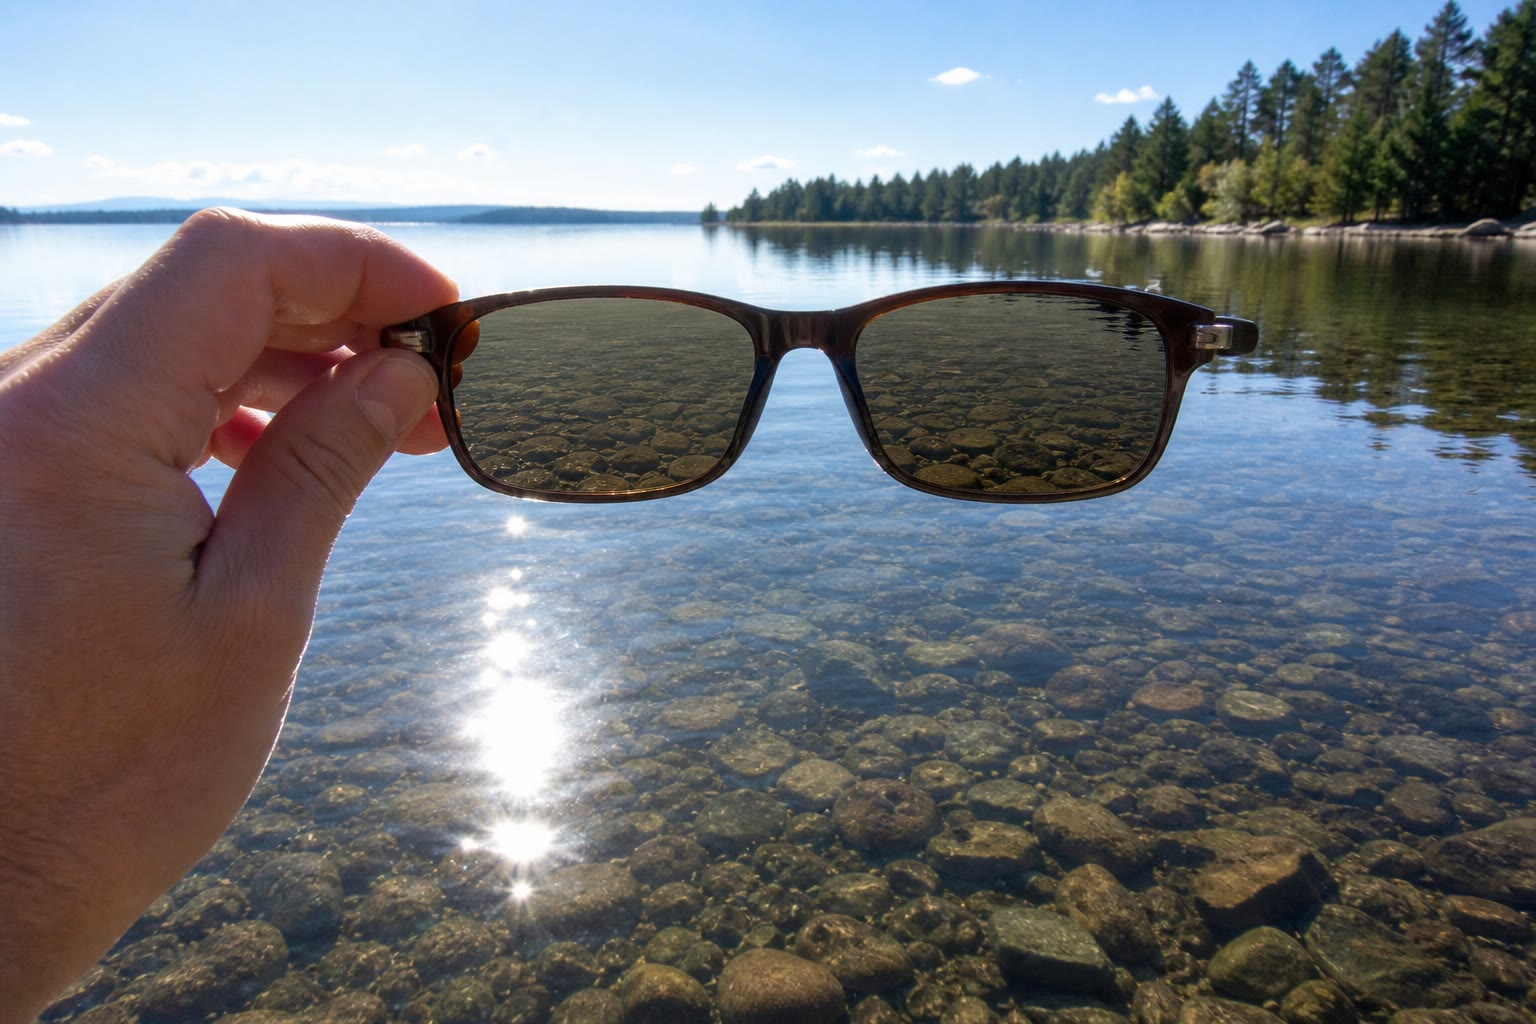
\includegraphics[width=0.58\linewidth]{images/book4/ai/b4-13-polarizing-sunglasses-lake.jpg}

{\small Polarizing sunglasses held before a lake: the glare, reflected near Brewster's angle and polarized horizontally, is cut by the vertical transmission axis of the lenses, and the lake bed shows through.}
\end{omfigure}

\section{Problem: The wave, the screen and the sail}

\begin{problem}[{Weekend problem --- a laser beam taken apart into its
fields, a screen that paints with polarization, and a spacecraft that
sails on light}]
\label{pb:b2:plane-waves-polarization:1}

\medskip
\noindent\textbf{Part I --- The beam.}
A helium--neon laser emits \qty{10}{mW} at \qty{632.8}{nm} in a beam of
\qty{1.0}{mm} diameter, linearly polarized along $x$, travelling along
$z$.
\begin{enumerate}
  \item Frequency, wavenumber, photon energy; photons emitted per
        second.
  \item Intensity; amplitudes $E_0$ and $B_0$; write $\vect E(z, t)$ and
        $\vect B(z, t)$.
  \item Energy density (mean) and the energy contained in \qty{1}{m} of
        beam; how long is the beam emitted in \qty{1}{ns}, and how many
        wavelengths does it contain?
  \item \omterm{thm:b2:poynting-vector:poynting}{Poynting vector}: mean value and its oscillation; momentum
        carried per second; force on a black target and on a mirror.
  \item Compare $E_0$ with the field that binds the electron in a
        hydrogen atom (\qty{5e11}{V/m}) and $B_0$ with the Earth's field
        (\qty{50}{\micro T}).
  \item \omterm{prop:b2:poynting-vector:wave}{Radiation pressure} on a black beam stop, in pascals.
  \item A free electron placed in the beam: amplitude of its velocity
        oscillation in the electric field (neglect the magnetic force
        first); ratio of the magnetic to the electric force on it ---
        why is the magnetic force negligible for matter in ordinary
        light?
  \item Write the fields of the same beam if it were circularly
        polarized; what changes in the intensity, in the \omterm{thm:b2:poynting-vector:poynting}{Poynting
        vector} and in its time dependence?
  \item The beam passes through a polarizer whose axis makes
        \qty{30}{\degree} with $x$: transmitted power; then through a second
        one crossed with the first: power; insert between them a
        third at \qty{45}{\degree} from the first: power.
\end{enumerate}

\medskip
\noindent\textbf{Part II --- The screen.}
A liquid-crystal screen: backlight (\omterm{def:b2:plane-waves-polarization:states}{natural light}), a polarizer, the
cell, a crossed polarizer. With no voltage the cell rotates the
polarization by \qty{90}{\degree}; with voltage it does nothing.
\begin{enumerate}[resume]
  \item Fraction of the backlight's intensity transmitted in the
        bright state (perfect polarizers); in the dark state.
  \item An intermediate voltage makes the cell behave as a retarder
        of phase $\delta$ between its axes, which are at \qty{45}{\degree} to the
        polarizers (no rotation): show that the transmission is
        $\sin^2(\delta/2)$ --- the grey scale.
  \item Viewed through a polarizer rotated to \qty{90}{\degree} from the
        screen's output polarizer, what is seen? At \qty{45}{\degree}?
  \item A \omterm{prop:b2:plane-waves-polarization:plates}{quarter-wave plate} glued on the screen at \qty{45}{\degree} to its
        polarizer turns the output circular: advantage for a viewer
        wearing polarizing sunglasses?
  \item Perfect polarizers would pass half of the backlight in the
        bright state; real sheets transmit $85\%$ of the ideal each, and
        the colour filters of a pixel pass a third of the light:
        fraction of the backlight's power reaching the viewer in white;
        name the two places where most of the light is lost.
  \item Real crossed sheets leak $0.1\%$ of the light: contrast ratio
        of the screen (bright over dark) in the dark room.
  \item Photographers' "circular polarizers" are a linear polarizer
        followed by a \omterm{prop:b2:plane-waves-polarization:plates}{quarter-wave plate} at \qty{45}{\degree}: what does
        the camera receive, and why is that better for the
        polarization-sensitive beam splitter of its autofocus than
        linear light?
  \item Why do 3D-cinema glasses use circular rather than \omterm{def:b2:plane-waves-polarization:states}{linear
        polarization}? What happens to the crosstalk between the eyes
        if the viewer tilts the head by \qty{20}{\degree} with linear
        glasses (intensity leaking into the wrong eye)?
\end{enumerate}

\medskip
\noindent\textbf{Part III --- The sail.}
A solar sail of area $S = \qty{1000}{m^2}$ and total mass $m = \qty{50}{kg}$,
perfectly reflecting, at $D = \qty{1.0}{au} = \qty{1.5e11}{m}$ from the Sun
($I = \qty{1.36}{kW/m^2}$; Sun's gravity \qty{5.9e-3}{m/s^2} there).
\begin{enumerate}[resume]
  \item Radiation force when the sail faces the Sun; acceleration;
        ratio to solar gravity.
  \item The sail is tilted by $\theta$ from facing the Sun: show that the
        force is normal to the sail and proportional to $\cos^2\theta$
        (intercepted power $\times\cos\theta$, momentum change along the
        normal $\times\cos\theta$).
  \item To spiral outward the sail keeps a force component along its
        orbital velocity: for $\theta = \qty{35}{\degree}$, tangential
        acceleration; speed gained per year; compare with the Earth's
        orbital speed (\qty{30}{km/s}).
  \item Why does the same sail, near Mercury ($D = \qty{0.39}{au}$), get
        $6.6$ times the force, and why is the ratio to gravity
        unchanged?
  \item The sail's film is \qty{2}{\micro m} of aluminized plastic: its
        temperature in sunlight if it absorbs $10\%$ and radiates from
        both faces as a black body ($\sigma = \qty{5.67e-8}{W.m^{-2}.K^{-4}}$).
  \item Time needed to gain \qty{1}{km/s} facing the Sun; what would an
        absorbing (black) sail of the same size achieve?
  \item Check the momentum of light with photons: number of photons
        hitting the sail per second (\qty{2}{eV} average) and the
        momentum $hf/c$ of each; recover the force.
  \item Sum up: the three quantities carried by the wave (energy,
        momentum, polarization) and the device of this problem that
        exploits each.
\end{enumerate}
\end{problem}
